\documentclass[letter, USenglish, 11pt, subfigure]{article}
\usepackage[margin=1in]{geometry}
\newcommand*{\ATLASLATEXPATH}{./}
\usepackage{\ATLASLATEXPATH atlaspackage}
\usepackage{\ATLASLATEXPATH atlasbiblatex}
\usepackage{\ATLASLATEXPATH atlasphysics}
% \usepackage{\ATLASLATEXPATH atlasjetetmiss}
\usepackage{\ATLASLATEXPATH ANA-SUSY-2018-12-PAPER-defs}
\usepackage{enumerate}
\newcommand{\mm}{\ensuremath{\mu^{+}\mu^{-}}}
\newcommand{\bsmm}{\ensuremath{\Bs\to\mm}}
\newcommand{\bdmm}{\ensuremath{\Bd\to\mm}}
\usepackage{lineno}
%\linenumbers
\usepackage{wrapfig}
\usepackage{placeins}
\usepackage{pdfpages}
\usepackage[none]{hyphenat} 
\addbibresource{proposal_WHopkins.bib}
\addbibresource{ATLAS-SUSY.bib}

\pagestyle{headings}

\title{Early Career Research Proposal: \\Machine-Learning-Driven New Physics Searches at the Large Hadron Collider}
\author{Applicant/Institution: Walter Hopkins, Argonne National Laboratory\\ Postal Address: \\Argonne National Laboratory, 9700 S. Cass Avenue, Building 360, Lemont, IL 60439
  \\PI name: Walter Hopkins\\Position title for PI: Assistant Physicist\\PI telephone number, email: (630) 252 7551, whopkins@anl.gov\\Administrative Point of Contact name, telephone number, email:\\Barbara Freeman, (630) 252-8145, bfreeman@anl.gov\\FOA Number: DE-FOA-0002421\\DOE/SC Program Office: HEP\\ Topic Area: Experimental Research at the \\Energy Frontier in High Energy Physics\\DOE/SC Program Office Technical Contact: Abid Patwa\\Year Doctorate Awarded: 2013\\Number of Times Previously Applied: 1\\Eligibility Extension Requested: No\\Signature of Laboratory Director: \\ \\ \\Paul K. Kearns, Laboratory Director
}
\date{}

\begin{document}
\pagenumbering{gobble}
%\includepdf{Hopkins_coverPage_proposal.pdf}

%\maketitle
\clearpage
\tableofcontents
\clearpage
\pagenumbering{arabic} 
% NOTES BASED ON COMMENTS RECEIVED
% 1. Clustering
% a. Make clear that clustering will guide us to a region we will manually develop.
% b. Highlight the connection between sim (gen, and reco) and clustering.
% c. Mention that there may well be no new signal regions but we need to test this to be sure, both with pMSSM and potentially the SMEFT.
% d. Find example where a standard analysis has missed something but clustering has not. (somewhat of a chicken and egg problem...)
% e. Mention the challenges in estimating backgrounds (even in the intro)
% f. Mention the connection with the broader pMSSM studies.
% g. Connection with reinterpretations?
% h. What kind of resources are needed? Give something quantifiable.


% 2. Geant4
% a. Emphasize the physics connection between FullSim and background estimation.
% b. Mention how this is part of a broader ATLAS effort.
% d. Understand the choice of the current range cut in ATLAS.
% e. Maybe omit the geometry discussion.

% 3. Miscellaneous
% a. Highlight how you will work with students who could benefit from ML (maybe mention OK)
% b. Maybe include support for students instead of the 21K computer (which is no longer needed).
% c. Give more details about alternative methods for both projects.
% d. Highlight how I will use the lab's ML expertise, together with the computing resources.
% e. More details about my ML experience.
% Mentoring, Workforce Development, and DEI
% eBUD proposal ID: 38588.1
\section{Introduction}

Results from the Large Hadron Collider (LHC) experiments have verified the predictions of the highly successful Standard Model (SM). However, the SM  lacks an explanation for several observed phenomena (e.g., dark matter) motivating the search for Beyond the Standard Model (BSM) physics. The current BSM search strategy uses simplified BSM models~\cite{simpModels} (i.e., models with 2-5 parameters) to design BSM search regions. This simplified approach was driven by enhanced BSM physics sensitivity from the large increases of center-of-mass energies during early LHC upgrades. Future LHC upgrades will no longer include significant increases in energy, but will first result in a doubling (Run~3) and then a tenfold increase (HL-LHC) of the current data set.

The HL-LHC comes with challenges; in particular, two challenges faced by the ATLAS experiment are (1) the need to exhaustively probe the large high-dimensional data set (where the dimensions are experimental observables such as particle momenta) for evidence of BSM physics and (2) the computational requirements of producing large amounts of simulations to estimate SM backgrounds for BSM physics searches using semi-data-driven methods. This proposal presents {\bf the development of machine learning (ML) algorithms to both methodically identify new BSM searches and enable accurate background simulations for these searches.} The increase in High Performance Computing (HPC) resources (e.g., the upcoming Aurora supercomputer, for which the PI is leading an early access proposal) yields a unique opportunity for facing these challenges.

The lack of evidence for BSM physics motivates a change in search strategy, specifically to move beyond using simplified theory models to design searches. Broader frameworks, e.g., the 19-parameter Phenomenological 
Minimal Supersymmetric Standard Model (pMSSM)~\cite{Djouadi_2007,Berger:2008cq,Cahill_Rowley_2012}, have been studied but have not been used to build a BSM search program. This is because they can produce thousands of models and applying the current labor-intensive search methodology at such a scale is not feasible. Previous attempts at categorizing the experimental observables of these models only included $\sim$10 models. This proposal presents {\bf the development of a novel search strategy for the HL-LHC based on probing the experimental observables of thousands of models with ML techniques.} The PI will develop the ML-driven search strategy in the context of ATLAS Supersymmetry (SUSY)~\cite{Golfand:1971iw,Volkov:1973ix,Wess:1974tw,Wess:1974jb,Ferrara:1974pu,Salam:1974ig} searches, but the strategy could be applied to other models and experiments. The PI's experience in ML, starting with the use of ML for his Ph.D. thesis~\cite{Aaltonen:2011fi,Aaltonen:2013as}, will aid the success of this proposal. The PI will also draw from his work within the ATLAS SUSY group, both as a leader of flagship searches~\cite{stop0L_1,stopRun1,stop0L_2,stop0L_3} and as a subgroup convener of the ATLAS SUSY strong production group, to ensure the new search strategy is validated and ready to guide the physics search program for the HL-LHC. Additionally, the PI will leverage the computing resources and ML expertise at the Argonne Leadership Computing Facility (ALCF).

An important aspect of designing BSM search regions is the estimation of SM backgrounds with semi-data-driven methods which require accurate simulations. ATLAS uses two frameworks for detector response simulations: a fast parameterization (FastSim)~\cite{ATL-SOFT-PUB-2018-002} and an implementation of \GEANT~\cite{Agostinelli:2002hh} (FullSim). The scale of the computational cost for the required SM background simulations at the HL-LHC prohibits the use of FullSim~\cite{computingCDR}, and FastSim has been shown to mismodel the decay products of heavy and energetic particles~\cite{AF3vCHEP2021}.% which are likely to be present in BSM physic searches.
Therefore, the PI {\bf proposes using ML as a way to utilize HPC resources for ATLAS detector simulations} by applying an ML-based correction to a modified configuration of FullSim, altered to be computationally faster. The use of an ML-based correction would allow for better use of HPC resources for simulation by performing the ML correction on graphical processing units (GPUs), which are expected to make up a large fraction of the computational power of future HPC resources. The success of the proposed work will be aided by the PI's experience with the ATLAS calorimeters and his work within the ATLAS \GEANT\ optimization task force, which studies computational bottlenecks of FullSim. 

\clearpage

\subsection{Background and Motivation}

Identifying new promising regions in ATLAS's experimental observable space (the space made up of all experimental observables, such as momenta of particles and invariant masses of combinations of particles) is essential in developing future BSM searches.
The current methodology of searching for BSM physics involves manually optimizing the requirements on observables for each simplified BSM model with a particular choice of two to three theoretical parameters (e.g., the masses of two BSM particles that are within reach of the LHC). More complex BSM models, such as the 19-parameter pMSSM (see Figure~\ref{fig:modelCartoon} for the relationship between the pMSSM and simplified models), have been studied by both ATLAS~\cite{ATLAS_pMSSM} and CMS~\cite{CMS_pMSSM}. These studies involved scanning the 19 theory parameters, simulating the physics processes that result from a particular choice of parameters, applying simplified detector effects, and evaluating whether a particular set of theory model parameters was excluded by previous ATLAS or CMS searches. The non-excluded models were studied further to understand why they evaded previous searches. Within ATLAS, some of these models had their mass spectra manually inspected (an example mass spectrum of such a model is shown in Figure~\ref{fig:cms_pMSSM}a) to gain insight into their expected signature in experimental observable space. This method resulted in some additional interpretation of standard early Run~2 SUSY searches~\cite{stopEarlyRun2}. However, the experimental space of the non-excluded models was not systematically probed and no new searches were designed on the basis of the non-excluded models due to the difficulty of interpreting thousands of models manually. CMS attempted to interpret the non-excluded models as a function of average values of observables as shown in Figure~\ref{fig:cms_pMSSM}b. This figure yields valuable information about the observables of non-excluded models, but is difficult to interpret because of the high dimensionality of the observable space. 
\begin{figure}[!htbp]
  \centering
  \subfigure[Relationship of simplified models (with 2-5 parameters) and broader models (19-parameter pMSSM) in theory parameters space.]{\includegraphics[width=0.45\textwidth]{figures/modelCartoon.pdf}}
  \hspace{3mm}
  \subfigure[Illustration of how a simplified model and broader models (pMSSM1-4, representing four sets of theory parameters) could populate experimental observable space. ]{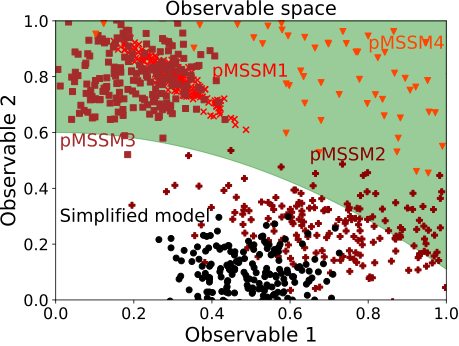
\includegraphics[width=0.45\textwidth]{figures/expSpaceSimplified.pdf}}
  \caption{Current SUSY searches are designed using simplified models (a, right) which have 2-5 parameters (e.g., masses of the BSM particles), which are only a small part of broader models such as the pMSSM (a, left). Broader models may populate unprobed regions of observable space (b, green shaded area), but constructing search regions using broader models is difficult with the current search-region design paradigm. Clustering, a group of ML algorithms, would allow for a more automated approach that would facilitate search-region design for broader theories such as the pMSSM.}
  \label{fig:modelCartoon}
\end{figure}

\begin{figure}[!htbp]
  \centering
  \subfigure[ATLAS interpretation of non-excluded pMSSM models.]{\includegraphics[width=0.4\textwidth]{figures/spectrum_pMSSM.pdf}}
  \subfigure[CMS interpretation of non-excluded pMSSM models.]{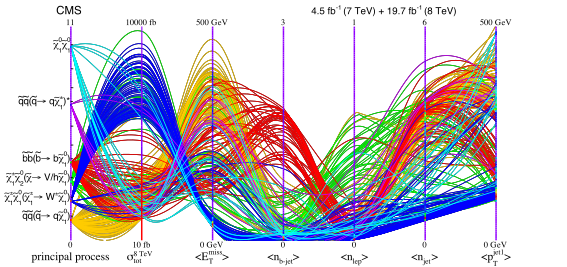
\includegraphics[width=0.59\textwidth]{figures/cmsPMSSMObservables.pdf}}
  \caption{\label{fig:cms_pMSSM} ATLAS (a) and CMS (b) interpretations of non-excluded pMSSM models after Run~1. The ATLAS interpretation involves manually inspecting the particle mass spectrum for each model (of which there were thousands) to predict the experimental signature. Each line in (a) corresponds to a particle mass, while the arrows indicate decays. The CMS interpretation considered averages of experimental observables. Each curve in (b) represents a non-excluded model, while the y-axis shows the value of the average of various observables listed on the x-axis. Despite only showing five observables, this representation of non-excluded models is difficult to interpret. ML is adept at summarizing high-dimensional data and will allow for the automatic interpretation of many models by grouping models together in regions of observables space which would form proto-search regions.}
\end{figure}
% Mention inputs and outputs clearly
Systematically probing the observable space of non-excluded models, which could be harboring new physics, requires novel techniques that are able to summarize high-dimensional spaces. Machine learning is especially adept at processing high-dimensional spaces and can be used to identify promising new search regions inspired by broad theory models such as the pMSSM. In particular, ML clustering algorithms, which group similar data points together, could group thousands of pMSSM models with different theory parameters but similar experimental signatures, forming the basis for new search regions. Considering the large number of models, identifying proto-search regions on the basis of these models is simply not practical with previous methods. Additionally, ML's ability to derive high-level features, such as particle masses from daughter particle momenta, makes it an attractive approach for automatically designing new proto-search regions using common low-level features. Thus ML has the potential to expand BSM searches for the HL-LHC by guiding the searches in an automated and methodical way. The identified proto-search regions would then be studied further and (semi)-data driven background estimates would be developed to build a robust BSM search.

Owing to the scale of both the simulations needed for the clustering and the clustering itself, this proposal will take advantage of advanced computing resources such as HPC resources. Argonne National Laboratory has both computing expertise (at the ALCF) and resources (e.g., Aurora) that will make the realization of this proposal possible. Significant computing resources will be required for automated feature extraction and to cluster the samples from the large number non-excluded pMSSM models. Additionally, the determination of the type of clustering algorithm and the optimal parameters for the clustering algorithm may require several passes through this large data set. The PI's team, consisting of two postdocs and himself, and university collaborators (students, postdocs, and advisors) will build on the existing relationship with ALCF experts to scale and optimize to both develop and optimize clustering algorithms.

BSM physics, that could be hiding in regions identified by clustering, is likely to include W/Z/Higgs boson or top quark decays, which can be mimicked by SM processes. These decays can be identified as jets (objects that represent the products of quark and gluon hadronization) with particular correlations between the jet constituents (substructure). Thus, for BSM physics searches, the modeling of substructure is crucial in estimating SM backgrounds accurately.

Although significant advances have been made to improve the modelling of the parametric FastSim~\cite{AF3vCHEP2021}, it has been shown to still mismodel the jet masses in substructure for certain BSM decays. The effect of this mismodeling on the W boson candidate mass can be seen in Figure~\ref{fig:wMass}~\cite{AF3vCHEP2021}, which compares the mass in FastSim version 2, FastSim version 3, and FullSim. There have been recent efforts to develop ML simulation, based on generative adversarial networks (GAN) and variational autoencoders, that would completely replace FastSim ~\cite{calogan,atlasgan}. These efforts show promise and actually improve the modeling of heavy particle decays somewhat. However, challenges remain in modeling as well as in aspects such as training (GANs are notoriously difficult to train) and interpretability. Thus, to maximize the discovery potential for BSM physics at the HL-LHC, some use of FullSim to simulate SM background for semi-data-driven methods will be required. 

\begin{wrapfigure}{L}{0.5\textwidth}
  \centering
  \includegraphics[width=0.5\textwidth]{figures/af3_jetmassR10.pdf}
  \caption{\label{fig:wMass} Comparison between Geant4, FastSim version 2, and FastSim version 3 of the mass of leading (in $\pt$) trimmed jets with jet radius parameter of 1.0 for a $W'\to WZ \to 4q$ sample~\cite{AF3vCHEP2021}. Although FastSim version 3 has improved modeling of this variable, it still deviates significantly from Geant4. }
\end{wrapfigure}

% Need to rephrase this to make clear that new computing resources are needed and GPU usage makes that possible. Should also emphasize that some search regions will still require fullsim and we shouldn't limit our physics due to the lack of good simulation.
However, producing simulations with FullSim for HL-LHC conditions with sufficient statistics is computationally prohibitive with current CPU-based resources. New types of resources, such as the Aurora HPC which could cover ATLAS' simulation computing needs with only $\sim$3\% of its computing power, need to be utilized and/or significant processing speed improvements to FullSim are required to meet budget constraints (see Figure~\ref{fig:currentComputing})~\cite{computingCDR}. One of the main computationally expensive parts of the ATLAS simulation is the simulation of particles navigating through the complex geometry of the EM calorimeters~\cite{Muskinja:2753974}. Computational speed improvements can be achieved by eliminating particles (and thus their daughters) by tuning FullSim configurations. The reduction in simulated particles would remove many of the geometric calculations and reduce computing time.
As an illustrative example of the computing power of future HPCs, consider Aurora, which, with its expected exaflop of computing power, would on be 
The gains in computational speed from changing FullSim configurations typically reduce the accuracy of the simulation. This proposal aims to develop an ML-based correction to a faster FullSim configuration to ensure a minimal loss in accuracy. The ML-based correction algorithm can be run on a variety of computing resources such as future HPC resources. These resources will have significant fractions of compute power in the form of GPUs. Utilizing GPUs typically requires rewriting code, such as \GEANT, but an ML algorithm can exploit GPUs since ML libraries (such as TensorFlow~\cite{tensorflow2015-whitepaper} and PyTorch~\cite{NEURIPS2019_9015}) are already optimized for a variety of computing resources. Thus, the proposed work could make more computing resources available (CPU and GPU) for simulation (currently FullSim is only utilizing CPU resources), potentially allowing for the needed amount of FullSim for new physics searches at the HL-LHC. 

 

\begin{figure}[!htbp]
  \centering
  \subfigure[CPU usage by task.]{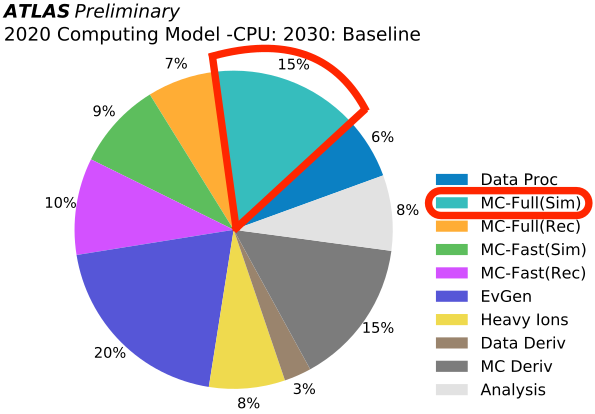
\includegraphics[width=0.45\textwidth]{figures/CPU_PieChart_baseline.pdf}}
  \subfigure[Projected CPU usages as a function of time.]{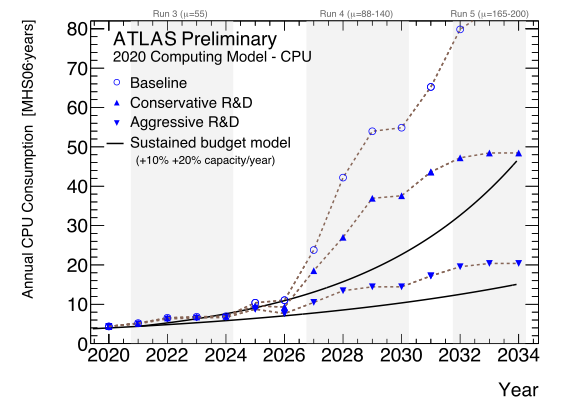
\includegraphics[width=0.45\textwidth]{figures/cpuHLLHC_comparison_2020_InputData_3April_ATLAS.pdf}}
  \caption{\label{fig:currentComputing} Projected CPU usage by ATLAS task (a) and as a function of year (b)~\cite{computingCDR}. FullSim currently takes up 15\% of the ATLAS computing budget, an infeasible fraction in the HL-LHC era, as shown in (b) as the baseline scenario (hollow circles), which is well above the budgetary constraints (shown as solid black lines). The simulation of the EM calorimeters makes up 58\% of the FullSim computational cost. The cost of the EM calorimeter simulation can reduced by tuning FullSim configurations (which will reduce accuracy) and then correcting for any changes in final physics quantities with ML.}
\end{figure}

\section{Project Objectives}
The objective of the proposed work is to develop clustering algorithms to methodically design a BSM search strategy for Run~3 and the HL-LHC. The ongoing Run~2 pMSSM scan, which is expected to conclude in early 2023, yields a unique opportunity to identify new BSM search regions for Run~3. To enable these searches for the HL-LHC, the proposed research also aims to prepare FullSim for HL-LHC conditions by improving the computational speed of FullSim and making use of future HPC resources. The specific objectives are as follows:
\begin{itemize}
\item Develop an ML-driven BSM physics search strategy.
  \begin{itemize}
  \item Apply clustering to non-excluded models resulting from the ATLAS Run~2 pMSSM scan and identify promising regions for further development into new search regions for Run~3. The clustering algorithm will commonly used human-developed high-level variables as inputs. 
  \item Introduce automatic high-level variable (e.g., invariant di-particle masses) extraction to clustering. The aim is to mitigate the chance that BSM physics is missed because of the use of suboptimal high-level variables. %Prepare to drive search strategies for the HL-LHC by further automating the approach with feature extraction.
  \end{itemize}
\item Prepare the ATLAS detector simulation to produce high-statistics SM background simulations for HL-LHC BSM searches.
  \begin{itemize}
  \item Develop an ML-correction algorithm on detector geometries with incrementally increasing complexity.
  \item Validate the ML-correction algorithm and integrate it into the ATLAS simulation workflow.
  \end{itemize}
\end{itemize}

\section{Proposed Research and Method}

\subsection{ML-driven BSM Physics Search Strategy}

The goal of applying clustering in experimental observable space (made up of particle momenta, combined masses, etc,) is to methodically identify undercovered or unprobed regions of observable space. These unprobed regions could then be studied further for their potential for BSM physics discovery. Broad theoretical models, such as the 19-parameter pMSSM, can be used to populate experimental observables space with Monte Carlo (MC) simulations. After models that have already been excluded by previous experimental results are removed, these models would populate regions of high-dimensional experimental observables space that previous searches missed, thus yielding an opportunity for new searches. These promising regions can then be ordered by their distance from SM backgrounds (which can be added to the clustering inputs) to identify regions with the highest potential for BSM physics discovery.  A sketch of the proposed clustering workflow is shown in Figure~\ref{fig:clusteringWorkflow}. Once a set of regions has been selected, further studies can be performed to assess the viability of robustly estimating SM backgrounds for these regions with (semi-) data-driven methods (these studies would address questions such as: can a control region with sufficient data statistics be designed?).

The proposed research will summarize regions in observable space with clustering algorithms, increasing the complexity of the algorithms incrementally. Clustering will initially be applied to the ongoing ATLAS Run~2 pMSSM scan, which is aiming for a result at the end of 2022, using experimental observables commonly used in SUSY searches as inputs (particle momenta, missing transverse energy, etc,). The regions found by clustering will then be used by the PI's team to develop a new BSM search for Run~3 (which is projected to start in 2022), with a publication expected in 2024. The final result of the proposed research will yield an automated method to construct new BSM proto-search regions in preparation for the HL-LHC start in 2027-2028.

\begin{figure}[!htbp]
  \centering
  \subfigure[Theory parameter space]{
    \includegraphics[width=0.313\textwidth]{figures/theorySpace.pdf}
  }
  \subfigure[Observable space]{
    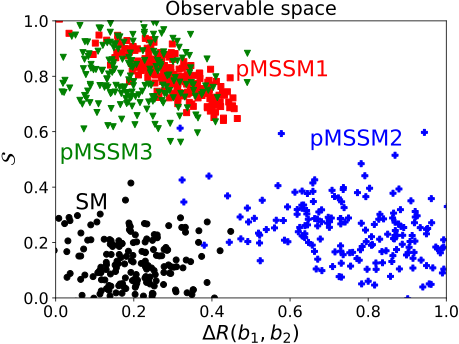
\includegraphics[width=0.313\textwidth]{figures/expSpace.pdf}
  }
  \subfigure[Clustering-produced regions]{
    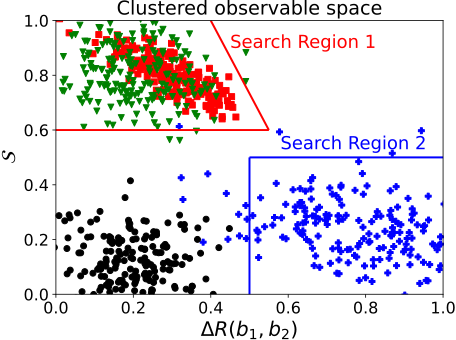
\includegraphics[width=0.313\textwidth]{figures/searchSpace.pdf}
  }
  
  \caption{Workflow for interpreting non-excluded pMSSM models with clustering in an example two-dimensional space. The two theory parameter values for four models (SM, pMSSM1-3) are shown in (a), while the space that these models populate in experimental observable space (filled with MC simulations of the models) is shown in (b) and (c). The two-dimensional space consists of two commonly used variables in ATLAS SUSY searches: the angular separation of two jets containing $b$-hadrons (\drbb) and missing transverse momentum significance ($\mathcal{S}$)~\cite{ATLAS-CONF-2018-038}. The variables have been scaled from 0 to 1, which is typical for inputs to ML algorithms. The result of clustering (c) is a set of proto-search regions that can be used to construct new BSM searches for Run~3 and beyond.}
  \label{fig:clusteringWorkflow}
\end{figure}

The first step, for the proposed work, is to apply a commonly used algorithm (outside of HEP) to an existing simplified theory model using kinematic variables implemented in current searches (similar to what is shown in Figure~\ref{fig:clusteringWorkflow}c). Several algorithms, such as $k$-means~\cite{kmeans} and density-based clustering~\cite{dbscan}, are currently being explored with the help of collaborators at the University of Oklahoma (a student and his advisor). The algorithm that both yields expected results on simplified models (based on regions designed in previous searches) and can be scaled up easily will be chosen. The algorithm will then be applied to the ATLAS Run~2 pMSSM effort to yield new search regions for Run~3. When applied to the Run~2 pMSSM scan, the clustering algorithm will make use of high-level variables (such as mass-based variables) which were manually designed. To prepare for searches in the HL-LHC era, the PI's team plans to study an additional layer of automation by investigating feature extraction before clustering, specifically using autoencoders to reduce the dimensionality of the input space to only the most pertinent features, to replace the myriad of manually designed and correlated variables used in the large number of existing searches. 

As an initial test, the PI has performed feasibility studies on an ATLAS result that searches for new physics in events with two top quarks and significant missing transverse energy in the all-hadronic channel (stop0L)~\cite{stop0L_3}. A simple two-dimensional space, consisting of two variables used in the analysis, was clustered using the $k$-means+gap statistic~\cite{Tibishirani} algorithm. Additionally, simulations of two BSM models (SUSY models) with different simplified model parameter values, resulting in different distributions of observables, were chosen. Finally, an SM background that was found to be dominant in the search was added to the data set. The results of using $k$-means to form clusters of these three theory models in the two-dimensional observable space are shown in Figure~\ref{fig:stopClustering} and demonstrate that $k$-means divides the observable space up in a reasonable way. The proposed regions do not perfectly contain each of the three models but this isn't expected (manually designed regions, of course, also display contamination from different simplified signal models and background) nor necessary since the final goal of the algorithm is to reduce thousands of models to a handful of promising regions.% to discriminate not only between the two BSM models but also between the BSM models and the SM background.

\begin{figure}[!htbp]
  \centering
  \subfigure[SUSY model 1]{\includegraphics[width=0.32\textwidth]{figures/complex_sig_1300_1_2DHist_postclustering.pdf}}
  \subfigure[SUSY model 2]{\includegraphics[width=0.32\textwidth]{figures/complex_sig_700_400_2DHist_postclustering.pdf}}
  \subfigure[SM Background]{\includegraphics[width=0.32\textwidth]{figures/complex_bkg_2DHist_postclustering.pdf}}
  \caption{Two-dimensional histograms of missing transverse momentum significance ($\mathcal{S}$) versus the angular separation of two jets containing $b$-hadrons (\drbb) for two BSM models, SUSY model 1 (a) and SUSY model 2 (b), and an SM background (c). The cluster boundaries are shown as the green lines for three clusters (shown as cluster 1-3) after applying $k$-means clustering. Both variables have been scaled to have values between 0 and 1. These distributions are an example of the two-dimensional space shown in Figure~\ref{fig:clusteringWorkflow}c (which shows a scatter version rather than a histogram), but for BSM models used in an ATLAS SUSY search~\cite{stop0L_3} using a two-parameter simplified model. Each SUSY model corresponds to unique values of the pair of parameters. The clustering algorithm identifies regions where each sample is dominant (cluster 1 for the SM, cluster 2 for SUSY model 2, and cluster 3 for SUSY model 2) and thus could be used as a basis for search regions to discover a BSM model.\label{fig:stopClustering}}
\end{figure}


\subsubsection{Run~2 pMSSM Clustering and Run~3 Searches}

Collaborators within the ATLAS SUSY group are in the process of performing a pMSSM scan based on the full Run~2 data set and will again identify models that evaded current search regions. To interpret and find new search regions from the result of the Run~2 pMSSM scan, the PI's team will first study the implementation of clustering on pMSSM models that were not excluded by ATLAS Run~2 searches. The ATLAS Run~2 pMSSM effort is expected to conclude by the beginning of Run~3 (late 2022 to early 2023) allowing the PI's team to study and develop clustering for new search-region identification. The results of clustering the observable space populated by non-excluded pMSSM models will then be used to find and start a new physics search for Run~3.

The PI's team will study the use of different clustering algorithms (e.g., the $k$-means algorithm, in combination with the gap statistic~\cite{Tibishirani} to determine the number optimal clusters) with commonly used observables such as lepton and jet momenta, $\met$, and large-R jets (which can identify top quarks and Z/V/H bosons). First, non-excluded pMSSM models with insufficiently high cross section ($<300~\ifb$) will be omitted from consideration. The ongoing pMSSM scan effort will produce MC collision data simulations of all scanned models with a simplified detector simulation (accurate simulations will only be necessary once a full BSM search region is designed with a semi-data driven technique to estimate background). The simulated data of non-excluded pMSSM models, as opposed to a summary statistic of the observable such as the mean of the observable, will then be used in clustering to ensure that effects that are in the tails of distributions are taken into account. This is a computationally expensive endeavor, owing to the number of models ($\mathcal{O}(10,000)$) and the number of simulated data points per model ($\mathcal{O}(10,000)$). Additionally, multiple clustering passes may be needed (e.g., for $k$-means with different numbers of clusters, $k$, to find the optimal $k$). The PI's team will leverage the HPC resources (e.g., Theta and ThetaGPU) and parallelization expertise that are available at the ALCF to prepare the clustering for pMSSM inputs.

As a contingency (if the previously explained method is too computationally intensive), a two-tiered approach to the interpretation can be applied. The clustering would first be applied to summary statistics of the observables, e.g., the averages, which would significantly reduce the computational scale of the clustering. Then, for clusters that are far enough away from the SM (based on simplified simulations), a clustering of the full data set can be performed to form proto-signal regions. 

To find clusters in experimental observable space to develop into signal regions, the clustering will initially be applied without SM background included. The main reason for leaving SM background out of the clustering for the Run~2 pMSSM scan is due to the computational challenge of producing enough background in regions populated by BSM models but not populated by current SM simulations. However, the reduction in regions to study (from $\mathcal{O}(10,000)$ to a handful), will already be a significant step towards interpreting the non-excluded models. The PI's team, given the PI's extensive experience in searching for BSM physics in regimes with high-energy decay products, will focus on developing search regions from clusters that include decay products from energetic top quarks or bosons. 

The final result of clustering of non-excluded pMSSM models could be a set of new searches for Run~3 that might otherwise not have been pursued. Thus, it is important that the proposed work be performed from late 2022 until 2023.

For future pMSSM scan (post Run~3 and beyond) SM background simulation could be included during clustering by iteratively generating and simulating backgrounds to populate all the probed regions of observable space. With SM backgrounds available clusters could be ordered by signal significance (with a metric such as S/B or the Asimov significance). The highest-ranking clusters will then be studied for further development. SM background simulations used in existing semi-data driven searches could be included in clustering initially and if the SM MC statistics are low, more background could be produced for that region. This computationally expensive procedure could be enabled by performing event generation and simulation on HPC resources. The PI is involved in studying how event generation can be performed on HPCs (as a lead of the ATLAS Aurora Early Science Project, together with collaborators from CERN and the ALCF) and described planned work enabling the use of Geant4 on HPCs as part of this proposal. 


\subsubsection{Automated High-level Feature Extraction for Clustering}
As mentioned in the previous section, selecting or developing high-level features that are important for grouping BSM models together is challenging. Many analyses use a wide set of variables that are highly correlated. Using all these variables with an algorithm such as $k$-means in an excessive number of clusters because of the diminishing power of distance measures as dimensionality increases. 

The PI proposes to address the challenge of selecting and developing high-level features by studying dimensionality reduction combined with clustering algorithms, specifically, autoencoders~\cite{BALDI198953}. Autoencoders are unsupervised (i.e., requiring no truth labels during training) NNs that aim to encode pertinent information from the input to a space with lower dimensionality by reconstructing the input from the encoded (or latent) low-dimensionality space and comparing reconstructed data with the original input. 
The general structure of an autoencoder is shown in Figure~\ref{fig:autoencoderDimRed}a. Once the autoencoder has been trained the encoder can be used to produce a low-dimensionality latent space that will be used as the input to a clustering algorithm such as k-means. 

The PI, with collaborators at the ALCF under a five-month Laboratory Directed Research and Development (LDRD) project, have developed and studied autoencoder algorithms to reduce the dimensionality for the stop0L signals. A simple autoencoder was trained to reduce $\sim$10 inputs to a one-dimensional latent space. The distributions of three signal points, two of which are expected to have similar signatures and one which is expected to have a unique signature, is shown in Figure~\ref{fig:autoencoderDimRed}b. The autoencoder was able to produce a latent space where signals were separated as expected. However, several challenges were identified by the team: the autoencoder training was unstable and occasionally the output of the autoencoder collapse to a single value (the average because a mean-squared-error loss was used during the optimization); the clustering and autoencoder were not simultaneously optimized which could result in a latent space which is suboptimal for clustering. Both challenges can be addressed with further studies into using autoencoders which add terms to the loss function to avoid learning trivial solutions (such as the average) and into methods for having a combined autoencoder+clustering loss. An example of an algorithm that the PI and his team hope to study is the use of variational autoencoders in combination with Gaussian model clustering~\cite{prasadVAEImageClus} which as the added benefit of yielding the number of clusters during the combined optimization.

\begin{figure}[!htbp]
  \centering
  \subfigure[Structure of an autoencoder]{
    \includegraphics[width=0.4\textwidth]{figures/Autoencoder_schema.png}
  }\hspace{3mm}
  \subfigure[One-dimensional latent space]{
    \includegraphics[width=0.48\textwidth]{figures/latentSpace_sig_700_400_allSignals_1DHist.pdf}
  }
  \caption{A schematic of the structure of an autoencoder network is shown in (a) while the latent space of an autoencoder trained on stop0L three signal points, two that have similar kinematics but different theory parameters and one that has unique kinematics, is shown in (b).}
  \label{fig:autoencoderDimRed}
\end{figure}


The autoencoder and clustering algorithms will need to be trained and applied to thousands of pMSSM models and may need to be optimized simultaneously, which will require significant computing resources. NN training is greatly accelerated by the use of GPUs since ML libraries are highly optimized for GPUs. Argonne will host several HPC resources, such as the Aurora supercomputer (for which the PI is leading the ATLAS Early Science Proposal) and Polaris, with significant compute power coming from GPUs. These Argonne resources, together with the collaboration with experts at the ALCF, wILL enable these complex algorithms to be run on thousands of non-excluded BSM models after Run~3. 

The PI's team will develop and test the autoencoder+clustering algorithm in time for use for the expected Run~3 pMSSM scan ($\sim$2025-2026). Clusters produced by the algorithm will be sorted by their background rejection power and studied further to develop semi-data-driven background estimates and to minimize/estimate systematic uncertainties. The most promising regions will be fully developed into new search regions for the HL-LHC.

% What about validation?
\FloatBarrier
\subsection{High-statistics and Accurate Backgrounds with ML}
The result of the clustering is likely to include proto-search regions that include the decay of energetic heavy objects such as Higgs/Z/W bosons and top quarks. To model these types of topologies accurately, the compute-intensive FullSim is required. Additionally, in the HL-LHC era large amounts of SM simulations are needed so that SM backgrounds and their systematic uncertainties can be assessed with semi-data-driven methods. ATLAS currently employs FullSim for most SM background MC but plans to substantially increase the use of FastSim to help address the HL-LHC computing challenges. However, to ensure an accurate description of certain regions of observable space (e.g., including decay products from heavy particles) for the HL-LHC era FullSim needs to be prepared for use on future heterogeneous computing resources (e.g., the upcoming Aurora supercomputer).

% FullSim, with the current computing model, is expected to use 15\% of ATLAS's CPU budget in 2030 (see Figure~\ref{fig:currentComputing}a). Considering the future budget projections and the increased CPU demands of the HL-LHC (see Figure~\ref{fig:currentComputing}b), FullSim needs to be modified to make use of future HPC resources to produce the amount of simulations needed for accurate background estimations.

\begin{wrapfigure}{L}{0.35\textwidth}
  \centering
  \includegraphics[width=0.35\textwidth]{figures/particleCostEMBPlusEMEC.pdf}
  \caption{\label{fig:compCostPie} Photons and electrons/positrons account for the largest fraction of the computational cost in the EM calorimeters. A large fraction of the simulation steps come from photons with energy less than 1 MeV as they navigate through the complex geometry of the EM calorimeters.}
\end{wrapfigure}

\GEANT\ simulates the interaction and movement of particles through a detector by taking steps through the detector volume, stochastically choosing what physics process, if any, to apply at each step. The number of steps, which is proportional to CPU usage, is not only determined by physics processes but also geometric boundaries (i.e., the more geometric boundaries exist, the more steps need to be taken). Studies have shown that the simulation of neutrons, electrons, and photons in the electromagnetic (EM) calorimeters is one of the most time-consuming part of FullSim (see Figure~\ref{fig:compCostPie}). This is mainly due to the geometrical complexity of the ATLAS EM calorimeters. There are ongoing efforts to reduce the time spent on simulating neutrons~\cite{nrr}, but as shown in Figure~\ref{fig:compCostPie}, three-quarters of the time is spent simulating electrons/positrons and photons. The PI's team plans to study an ML-based correction algorithm to mitigate any possible mismodeling resulting from modifications to FullSim configurations that improve the computational performance of FullSim (potentially up to a 15\% increase in speed). The combined ML correction and FullSim setup will then utilize upcoming HPC resources, which will make significant use of GPUs, more efficiently by evaluating the ML correction on GPUs while running FullSim on CPUs.

% Initial studies of photon propagation through the EM calorimeters, performed by the PI, have shown that the most common simulation process (95\% of all processes) that photons undergo in the EM calorimeters is transportation, i.e., simply moving through the geometry. The PI studied the use of ML to perform each geometrical navigation step, in an effort to speed up each step, but found that the inference time of even a simple ML algorithm ($\mathcal{O}$(ms)) was much longer than the \GEANT\ implementation for each step ($\mathcal{O}$($10\mu$s)). Similarly, replacing multiple consecutive transportation steps, of which there tend to be fewer than 50, with an ML algorithm was found to be infeasible. %These studies however did indicate that most photons have low energy ($<$ 1 MeV) and deposit most of their energy in the absorber of the calorimeter. 

An approach the PI is pursuing for this proposal is to limit the number of particles that are produced in the calorimeters, thus limiting the number of geometrical calculations needed. Existing parameters within \GEANT, known as production cuts, limit the number of particles produced during the EM calorimeter simulation. Production cuts impose a minimum energy requirement on secondary particles. If a particle is expected to produce secondaries that fall below the minimum energy requirement, no more secondaries are produced and instead the energy of the particle is deposited along the path of the particle until it has zero energy. These production cuts are set in units of length to account for different energy thresholds in different materials. 

ATLAS currently uses a production cut of 0.1 mm for electrons/positrons ($\sim$2.6 MeV for an electron in lead) % Needs to be checked
and is planning to use the same cut for photons in Run 3. Initial studies by the PI, using samples that are produced by shooting 20 GeV electrons at the EM calorimeter with production cuts ranging from 0.1 mm to 5 mm, have found that changing the production cut to 2 mm results in a reduction in running time of 15-20\%. The effect on the reconstructed $\pt$ of electrons as a function of production cut is shown in Figure~\ref{fig:simpleCorr}. For an ML algorithm to correct distributions of physics object (electrons, photons, etc) from a chosen production cut so that they resemble distributions from the default 0.1 mm production cut, the production cut must have a large-enough effect while not completely altering the distributions. A production cut of 2 mm would result in a change in properties of physics objects which is large enough to be corrected by an ML algorithm while delivering a 15-20\% reduction in computing time.

\begin{figure}[!htbp]
  \subfigure[CPU time for different production cuts]{\includegraphics[width=.5\textwidth]{figures/EMECvsRC_timing_El20GeV.pdf}}
  \subfigure[\pt\ for different production cuts]{\includegraphics[width=0.46\textwidth]{figures/pt.pdf}}
  \caption{\label{fig:simpleCorr}The CPU time relative to the default ATLAS value for production cut (0.1 mm, black dot) as a function of production (a) and the effect of production cuts on the \pt\ of reconstructed electrons (b).}
\end{figure}


\subsubsection{ML Algorithm R\&D and Optimization}
The PI proposes to tune the production cuts and to develop an ML algorithm to correct deposited energies resulting from the new production cut, ensuring that the final corrected simulation is accurate to within 10\% (FullSim typically agrees with data within this accuracy) of the ATLAS default value for production cuts. An ML-correction algorithm will first be developed for a simplified geometry and will then incrementally be improved to work with more complex geometries. The PI's team will use a simple one-dimensional calorimeter  (without lateral segmentation) example to produce a prototype of the correction algorithm which will correct the energy of all active gaps, using ML to match the total energy and shower depth of the default production cut. 

The stochastic nature of detector simulation makes training with matched data difficult, thus posing challenges to the use of regression. ML algorithms that will be explored include algorithms that reweight energy deposits with the output of a discriminator (which would be trained to discriminate between gaps with and without a modified production cut). The goal is to have at least a net 10\% improvement in running time, even without considering the added benefit of opening up the possibility of using resources that contain both CPUs and GPUs (FullSim currently only makes use of CPU resources).

Once the approach has been developed and its performance has been evaluated for the simple calorimeter geometry, more complex geometries will be explored. The more complex geometry will explore the effects of the production cut/correction combination on lateral shower shapes by extending the simple example along the lateral direction. The result of these studies will be published in a stand-alone paper. The PI's team will then continue developing a correction algorithm for the ATLAS calorimeter geometry.

Finally, the algorithm will be fine-tuned with a hyperparameter optimization for both inference time (to ensure improvements in the computational cost of the simulation) and accuracy (of the cell energies or related high-level quantities such as shower shape variables). The optimization of the final algorithm will greatly benefit from the hyperparameter optimization expertise and tools developed (such as DeepHyper~\cite{deephyper2,deephyper1}) at the ALCF.

\subsubsection{Validation and Integration into ATLAS Workflow}

Once the algorithm has been trained and tuned for optimal accuracy and computational cost, the ensemble effect of the algorithm (i.e., applying the algorithm to all of the EM calorimeters) will be validated by comparing particle showers produced with FullSim with particle showers where the algorithm was applied. Shower shape variables and physics quantities used at the analysis level, such as jet mass and substructure variables, will be used for validation.

Once the algorithm has been validated, the final ATLAS algorithm will need to be studied for optimal use of heterogeneous computing resources (resources that combine different processor architectures such as CPUs and GPUs). The number of events to which the correction algorithm is applied will need to be tuned to keep both CPU (which is the only resource FullSim can currently utilize) and GPU (which the ML-correction algorithm can utilize) resources busy. The collaboration that the PI has formed with ALCF parallelization experts as the PI of the Argonne ATLAS Aurora Early Science Proposal will be essential to this optimization effort. 

\subsection{Projected outcomes} 

This proposal aims to develop a novel systematic method of building a new physics search program which will be applied to ATLAS and the pMSSM, but could also be applied to any experiment and any broad theory model. The aim is to avoid missing a part of observable space that could have hints of BSM physics. The expected result for the beginning of Run~3 is a first application of clustering on non-excluded pMSSM models to prepare new Run~3 searches. Finally, for HL-LHC, the expected result is a new search based on pMSSM models that weren't excluded in Run~3 using more complex clustering that takes into account more of the available information. 

The proposed research is also expected to result in an increase in the computational speed of FullSim when simulating the ATLAS EM calorimeters. The proposed approach of using an ML algorithm to correct a fast FullSim configuration will allow for the more efficient use of HPC resources by the utilization of both GPU (by the ML-correction algorithm) and CPU (by FullSim) resources. Additionally, the computational speed improvement to FullSim alone could be as large as 15\%. It is expected that these improvements, after going through physics validation to ensure that the simulation accurately describes the data, would be implemented in time to be used for the HL-LHC in preparation of BSM searches developed by the clustering algorithm.

\section{Timetable of Activities}

The timetable of activities is shown in Figure~\ref{fig:timetable}. The first step in developing an automated search-region design algorithm is to use clustering with commonly used input variables to interpret the result of the ongoing Run~2 pMSSM scan. The Run~2 pMSSM scan is expected to finish near the beginning of calendar year 2023. The PI's team will first develop and test $k$-means clustering on the Run~1 pMSSM scan results while the Run~2 pMSSM scan is prepared is by a team of ATLAS collaborators. Once the scan is complete, the clustering algorithm can be applied to the new results, which will be published as part of the General Run~2 pMSSM paper (milestone 1 in Figure~\ref{fig:timetable}a). The result of clustering non-excluded Run~2 pMSSM models will point to several regions that can be further developed. The PI's team will develop one of these regions into a full (including semi-data-driven background estimates and systematic uncertainties) BSM search, which will result in the first publication (milestone 2 in Figure~\ref{fig:timetable}a) of a search based on a semi-automated search strategy. Near the completion of the Run~3 publication, the PI's team will focus on further automating the region designs by studying clustering in combination with feature algorithms, which will result in a publication on the development of the method (milestone 3 in Figure~\ref{fig:timetable}a).

Below is a summary of the milestones for the search-region design aspect of the proposal:
\begin{itemize}
\item Milestone 1: the publication of the Run~2 pMSSM scan results, which will include an interpretation of non-excluded pMSSM models using a common clustering algorithm in observable space.
\item Milestone 2: the publication of the results of a search based on the clustering of non-excluded pMSSM models.
\item Milestone 3: the publication of results for the R\&D on unsupervised feature extraction for a Run~3 pMSSM scan interpretation.
\end{itemize}

% Add description of timeline for G4 project
For the ML-correction algorithm for simulation, the first task will be to develop an ML algorithm to correct the effects of production cuts on a simplified geometry. The geometry will be based on the \GEANT\ B4 example, but extended to allow for the measurement of lateral shower shapes. The result of these studies will be published in a stand-alone (outside of ATLAS) publication, which is Milestone A in Figure~\ref{fig:timetable}b. The second task, which is expected to be more time-consuming, will be to expand the ML algorithm to correct the cells of the ATLAS EM calorimeters. As with the simplified geometries, the ML-based correction will be validated by comparing shower-shape variables. Milestone B will be a validated ML-correction algorithm that will be described in an ATLAS PUB note.
Below is a summary of the two milestones for the ML-correction algorithm aspect of the proposed work:
\begin{itemize}
\item Milestone A: publication on ML-correction algorithm developed for simplified geometries.
\item Milestone B: Validation of ML-correction algorithm within ATLAS.
\end{itemize}

\begin{figure}[!htbp]
  \centering
  \subfigure[Timetable for ML-driven search design.]{\includegraphics[width=.49\textwidth]{figures/clusteringTimetable.pdf}}
  \subfigure[Timetable for ML-based detector simulation correction.]{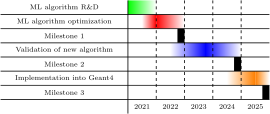
\includegraphics[width=.49\textwidth]{figures/geant4Timetable.pdf}}
  \caption{Timetable of tasks for the ML-driven search strategy R\&D (a) and for developing ML-based FullSim correction algorithms (b). The short-term goal is to apply clustering to the Run~2 pMSSM scan so that new search regions can be designed for Run~3. The clustering algorithm will then be refined so that it can be ready for use to exploit the large data set delivered by the HL-LHC.
    In parallel with the clustering R\&D, an ML algorithm that can correct deposited energies to incrementally more complex geometries will be developed. The aim is to have an algorithm that corrects a fast configuration of FullSim with a minimal loss of accuracy in time for use for background estimates needed by regions designed by the ML search-strategy algorithm at the HL-LHC.
  }
  \label{fig:timetable}
\end{figure}


\subsection{Personnel and Resources}
\label{sec:personnel}
The PI will lead a team to conduct the clustering and simulation efforts, which will consist of an average of 1.5 FTE of postdocs and 57\% of the PI's time. If received, the award will cover 100\% of the 1.5 postdocs' salary and 57\% of the PI's salary. For the first two budget periods, the PI's effort will be allocated to the proposed research at 0.64 FTE to cover some of the start-up effort while a postdoc is hired. For the remainder of the budget periods, 50\% of the PI's salary will be covered by the award.

Throughout the term of the award, the PI hopes to fund 0.5 FTE of an existing ATLAS postdoc. Additional effort, at 1 FTE, will come from a postdoc who is expected to start work about seven months into the first budget period (the time expected to be needed to hire a new postdoc). This postdoc's time would be split evenly between developing clustering and simulation algorithms. An additional postdoc, at 1 FTE, will be hired one year before the first postdoc's contract ends (after three years, during the beginning of budget period 4) and will continue until the end of budget period 5.

The PI will also investigate the possibility of working with graduate and undergraduate students on the proposed work with the aid of the DOE Office of Science Graduate Student Research program and the Science Undergraduate Laboratory Internships, respectively. Finally, Argonne's ATLAS Center, which hosts graduate students from local universities, yields another opportunity to work with graduate students on the proposed projects. 

Computing resources available at the ALCF include Theta and ThetaGPU until 2022 and Aurora in 2022 and onward. The resources are available to the PI in the form of Director's Discretionary Allocations, which are routinely granted to ECRP awardees who request allocations within certain specifications. Additional computing for smaller-scale testing will also be available through the Laboratory Computing Resource Center.

The PI's team expects to collaborate with \GEANT\ and ATLAS simulations experts, ATLAS SUSY group members, and ALCF computing experts. The PI has already initiated these collaborations by working within the ATLAS simulation optimization task force, leading SUSY analyses, and working with ALCF in the context of the Aurora ATLAS Early Science Proposal, respectively. 

\section{Summary}

The ATLAS collaboration has performed many searches for physics resulting from BSM phenomena. Despite this effort, no evidence for new physics has been found. As ATLAS moves into the high-luminosity era, which will result in a 20 times larger data set relative to the current data, novel and systematic methods are needed to find new search regions where new phenomena could be discovered. This proposal aims to develop such methods by studying ML techniques for automated BSM search region design using non-excluded theory models. These techniques could allow for search regions to be designed while taking thousands of theory models into account, as compared to a mere handful of models with current methodologies. The proposed approach will be incrementally improved: it will first be applied for Run~3 and then prepared to be more automated and to leave even fewer regions uncovered for the HL-LHC. 

To further maximize the discovery potential of the HL-LHC, this proposal presents an R\&D program aimed at improving the computational performance of the ATLAS calorimeter simulations with minimal loss in accuracy. These computational improvements are necessary to estimate backgrounds accurately at the scales required at the HL-LHC. These goals are planned to be achieved by tuning simulation parameters for faster computational speed but ensuring that the simulation accuracy is high with ML corrections. This combination of a faster FullSim, which will run on CPU resources, and an ML correction, which will run on GPU resources, will enable the efficient use of future HPC resources.

The success of this proposal will be aided by the PI's experience with BSM searches, the ATLAS EM calorimeter, and ML. The PI has led SUSY searches that involve probes in far reaches of observable parameter space and has performed physics performance studies for the ATLAS calorimeter upgrades. The PI has also studied ML algorithms for BSM searches as well as for approximating detector effects. Finally, the PI will draw from his experience as the lead for the Aurora Early Science Proposal, which aims at preparing ATLAS computing tasks to run on the Aurora supercomputer, to utilize HPC resources for improving both the BSM search strategy and background estimation at the HL-LHC.

The proposed work could result in a novel search strategy and accurate background simulations that would maximize the discovery potential of the HL-LHC. The ability to build search regions based on thousands of theory models and to accurately estimate SM backgrounds allows for a much more comprehensive understanding of theory model kinematics and a more comprehensive exploitation of the LHC data.

\clearpage
\appendix
\part*{Appendices}
\addcontentsline{toc}{part}{Appendices}
\section{Biographical sketch}
\subsection{Education and Training}
\begin{itemize}
\item Cornell University; Ithaca, NY; High Energy Physics, Thesis: ``Search for $\bsmm$ and $\bdmm$ Decays with  $10~\ifb$ of ${p\overline{p}}$ Collisions''; Ph.D.; 2013.
\item Cornell University; Ithaca, NY; High Energy Physics; M.S.; 2010.
\end{itemize}

\subsection{Research and Professional experience}
\begin{itemize}
\item 2018-present; Assistant Physicist at Argonne National Laboratory; Lemont, IL; working on SUSY searches and calorimeter simulations.
\item 2013-2018; Postdoctoral Research Assistant with University of Oregon; Eugene, OR and Meyrin, Switzerland (CERN); working on SUSY searches and the Liquid Argonne Calorimeters with the ATLAS experiment.
\item 2009-2013; Graduate Research Assistant with Cornell University; Ithaca, NY and Batavia, IL (Fermilab); working on rare $B$-meson decays at the CDF experiment.
\end{itemize}

% \clearpage
\subsection{Publications}
\begin{itemize}

\item ATLAS Collaboration, ``Search for a scalar partner of the top quark in the all-hadronic $t\bar{t}$ plus missing transverse momentum final state at $\sqrt{s}=13$~TeV with the ATLAS detector'', \href{https://arxiv.org/abs/2004.14060}{Eur. Phys. J. C 80, 737 (2020)}.

\item D. Benjamin, S. Chekanov, W. Hopkins, Y. Li, J. R. Love, ``Automated detector simulation and reconstruction parametrization using machine learning'', \href{https://arxiv.org/abs/2002.11516}{JINST 15 (2020) P05025}.

\item ATLAS Collaboration, ``Searches for third generation leptoquarks in $\rts=13\tev$ $pp$ collisions with the ATLAS detector'', \href{https://arxiv.org/abs/1902.08103}{JHEP 06 (2019) 144}.
  
\item ATLAS Collaboration, ``Summary of searches for dark matter and dark energy using $\rts=13\tev$ $pp$ collisions with the ATLAS detector at the LHC'', \href{https://arxiv.org/abs/1903.01400}{JHEP 05 (2019) 142}.

\item ATLAS Collaboration, ``Search for a Scalar Partner of the Top Quark in the Jets$+ \met$ Final State at $\rts=13\tev$ with the ATLAS detector'', \href{https://arxiv.org/abs/1709.04183}{JHEP 12 (2017) 085}.

\item ATLAS Collaboration, ``ATLAS Run 1 searches for direct pair production of third-generation squarks at the Large Hadron Collider'', \href{http://arxiv.org/abs/1506.08616}{Eur. Phys. J. C75 (2015) 510}.

\item ATLAS Collaboration, ``Search for direct pair production of the top squark in all-hadronic final states in proton-proton collisions at $\sqrt{s}=8$ TeV with the ATLAS detector'', \href{http://arxiv.org/abs/1406.1122}{JHEP 09 (2014) 015}.

\item ATLAS Collaboration, ``ATLAS Liquid Argon Calorimeter Phase-I Upgrade Technical Design Report'', \href{https://cds.cern.ch/record/1602230}{CERN-LHCC-2013-017}.

\item CDF Collaboration, ``Search for $B_s^0\to\mu^+\mu^-$ and $B^0\to\mu^+\mu^-$ Decays with CDF II Full Data Set'', \href{http://arxiv.org/abs/1301.7048}{Phys. Rev. D 87, (2013) 072003}, [Erratum: Phys.Rev.D 97, 099901 (2018)].

\item CDF Collaboration, ``Search for $B_s^0\to\mu^+\mu^-$ and $B^0\to\mu^+\mu^-$ Decays with CDF II'', \href{https://arxiv.org/abs/1107.2304}{Phys. Rev. Lett. 107 (2011) 191801}, [Addendum: Phys.Rev.Lett. 107, 239903 (2011)].

\end{itemize}

\subsection{Synergistic Activities}
\label{subsec:syn}
%\subsubsection{Leadership positions}
\begin{itemize}
\item August 2020-present: member of \GEANT\ optimization task force. % Add description
\item April 2020-present: SUSY strong production subgroup convener. % Add description
\item 2018-present: PI for the Argonne ATLAS Aurora Early Science Program.
\item 2014-2020: ATLAS SUSY stop search analysis team contact.
\item April 2020-present: Snowmass topical group convener for the Experimental Algorithm Parallelization group.
\end{itemize}

\subsection{Selected conference talks and seminars}
\begin{itemize}
\item November 2020: Pre-Learning a Geometry Using Machine Learning to Accelerate High Energy Physics Detector Simulations, Inter-experimental Machine-learning working group meeting, November 23, CERN.
\item November 2018: Jets and Machine Learning in ATLAS, ML4Jets 2018, Fermilab.
\item July 2018: Measurements with highly boosted top quarks using the ATLAS detector, BOOST 2018, Paris, France.
\item Fall 2016: Direct Stop Searches at ATLAS, Seminars at UC Davis, UC Santa Cruz, and Argonne National Laboratory.
\item June 2016: Third generation SUSY searches at the LHC, LHCP 2016, Lund, Sweden.
\item February 2016: Electronics Development for the ATLAS Liquid Argon Calorimeter Trigger and Readout for Future LHC Running, Vienna Instrumentation Conference (VCI) 2016, Vienna, Austria.
\end{itemize}

\subsection{Honors and Awards}
\begin{itemize}
\item 2021: LDRD Expedition Project Award: Developing unsupervised learning for use on Argonne's AI test beds.
\item 2014-2015: U.S. ATLAS Scholars Award.
\item 2009-2012: National Science Foundation Graduate Research Fellowship.
\item 2007-2008: Cornell Sage Fellowship, a Diversity Fellowship awarded by Cornell University on a competitive basis.
\end{itemize}

\clearpage

%\section{Current and pending support}
\includepdf[scale=.95,pages=1,pagecommand=\section{Current and pending support}]{cps_page2.pdf}

% Project/Proposal Title: ATLAS base. Energy frontier research at the ANL High Energy Physics Division. For the PI this includes new physics searches and work on simulations of high-energy collisions.\\
% Status of Support: current\\
% Proposal/Award number: KA2401041 and KA2101020\\
% Source of Support: DOE Office of Science, HEP\\
% Primary Place of Performance: Argonne National Laboratory, Lemont, IL\\
% Total Award Amount (including Indirect Costs): NA\\
% Person-Month(s) (or Partial Person-Months) Per Year Committed to the Project:
% \begin{enumerate}
%   \item Calendar year 2020: 12 months
% \item Calendar year 2019: 12 months
% \item Calendar year 2018: 3 months
% \end{enumerate}

\clearpage

\printbibliography
\clearpage

\section{Facilities and  other resources}
ANL offers various resources including office space for postdocs and potential students as well as several computing resources. The computing resources expected to be utilized include CPU and GPU resources available through the Laboratory Computing Resource Center. These resources are expected to be used to produce input data for ML algorithms for both detector simulation part of the proposed work as well as for initial studies for the BSM physics search strategy. The PI also plans to use computing resources at the ALCF, such as Theta, ThetaGPU and Aurora, via a discretionary allocation. These resources will be used for large scale training and optimization of the proposed research.

An additional important resource is the ATLAS experiment at the LHC at CERN. The PI's team will make use of ATLAS data and simulation for both projects and will occasionally travel to CERN to collaborate with CERN physicists.

Finally, for the development of ATLAS new physics searches, the PI's team will make use of the USATLAS Tier 3 computing resource.

\clearpage

\section{Equipment}
The requested funding will be used to purchase two laptops for the two postdocs that the PI will supervise. The combined cost of the two laptops is expected to be \$6,000.% a workstation containing at least two cards with general purpose graphical processor units (GPGPU). The cost of the workstation is expected to be  \$21,000 and will contain at least NVIDIA V100 GPGPUs. The workstation will be used by the PI's team for fast development and testing of machine learning algorithms. 
\clearpage

\section{Data management plan}
The majority of the data and code produced will come from the ATLAS experiment. ATLAS has its own data management plan which the PI's team will adhere to. The details of which can be found at \url{https://po.usatlas.bnl.gov/programoffice/datamanagementpolicy.php}.

Scientific results that used ATLAS data will be published in a scientific journal or an ATLAS publication note which will be publicly available on \url{https://arxiv.org/} and \url{https://twiki.cern.ch/twiki/bin/view/AtlasPublic/SimulationPublicResults}, respectively. Figures and tables will be made available in the same way as with other ATLAS results via HEPData (\url{https://www.hepdata.net/}) and ATLAS public pages. 

Additional data that is produced outside of ATLAS for initial ML algorithm development, will be stored on the ATLAS High Energy Physics divisional nodes in the HDF5 format and will consist of energy deposits in a simplified detector. The generated data is expected to be a small fraction of the available data storage on these nodes. Code and configurations used for the development of the algorithm and production of data will be kept at the Argonne Computing, Environment and Life Sciences (CELS) gitlab repository: \url{https://xgitlab.cels.anl.gov/}. Results from these studies, if published will be publicly available on \url{https://arxiv.org/}. 

\clearpage

\section{Other attachments}
% Put letters of collaboration here.

\end{document}
